\documentclass{article}[13pt]
\usepackage{graphicx}
\usepackage{geometry}
\usepackage{caption}
\usepackage{newtxtext}
\usepackage{newtxmath}

% Set custom page margins
\geometry{
  left=3cm,
  right=3cm,
  top=2.5cm,
  bottom=2.5cm
}

\begin{document}

\begin{titlepage}
    \centering
    \vspace*{5cm}
    {\Large Waseda University School of Political Science and Economices}\par
    \vspace{1cm}
    {\LARGE \textbf{Econometrics I Research Paper}}\par
    \vspace{1cm}
    {\Large LIEN YU HSIANG}\par
    \vspace{1cm}
    {\Large 1A202G34}\par
    \vspace{1cm}
    {\Large \today}\par
    \vspace{2cm}
\end{titlepage}

\section{Introduction}


\qquad This paper endeavors to conduct a thorough examination of the dataset `GSSdata2018.csv' through the application of statistical methods such as regression tests and hypothesis testing. The primary objective is to derive meaningful insights from the data, uncovering patterns and relationships that may exist. The use of robust statistical techniques ensures the reliability of our findings.
The `GSSdata2018.csv' dataset serves as the focal point for our analysis, with regression tests enabling us to explore connections between different variables. Additionally, hypothesis testing is employed to scrutinize specific assumptions, adding a layer of statistical rigor to our conclusions.
The intention is to delve beyond superficial observations, utilizing meticulous statistical analysis to reveal nuanced trends within the data. By employing reliable statistical testing methods, the paper aims to establish credible and insightful conclusions, contributing to a more comprehensive understanding of the dataset and facilitating the proposal of informed research outcomes.

\section{Data Description}

\qquad The dataset been utilized is `GSSdata2018', which is a dataset that made by 
nationally representative survey of adults in the United States conducted since 1972. 
And the dataset is publically avalible so anyone who wish to discover further insight can 
obtain the data. Before accessing the data through statistical means, it is important to fist look 
and summerized some basic but vital aspect of the data. 
\newline

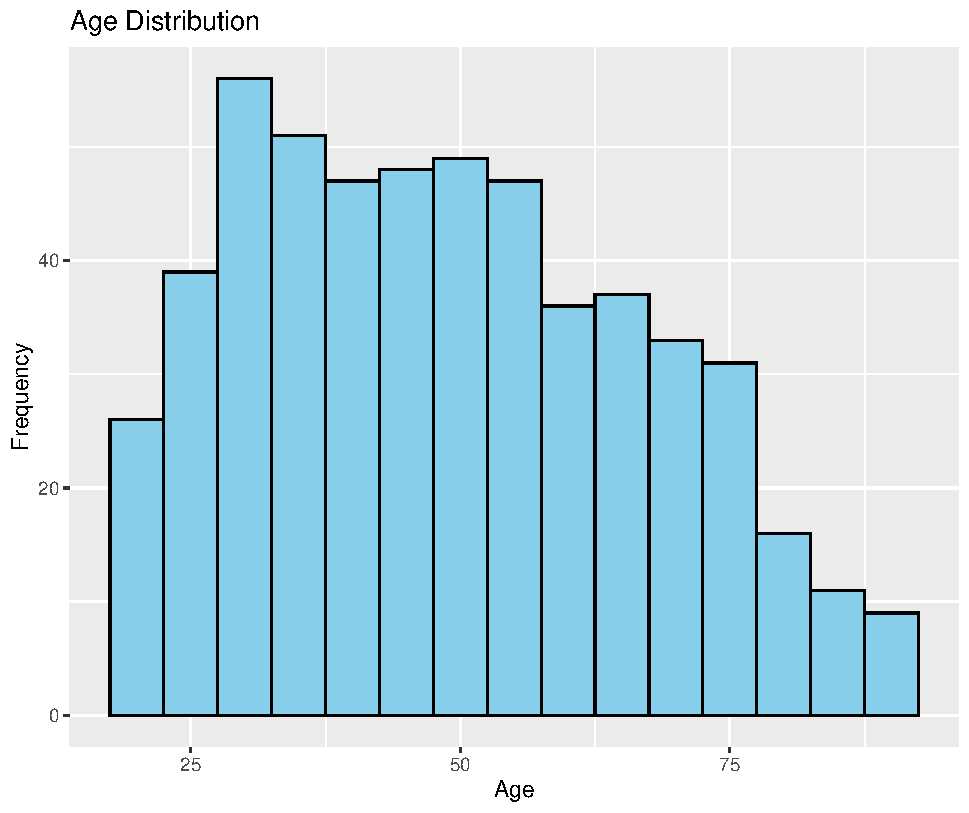
\includegraphics[width=0.4\textwidth]{1_age_distribution.pdf}
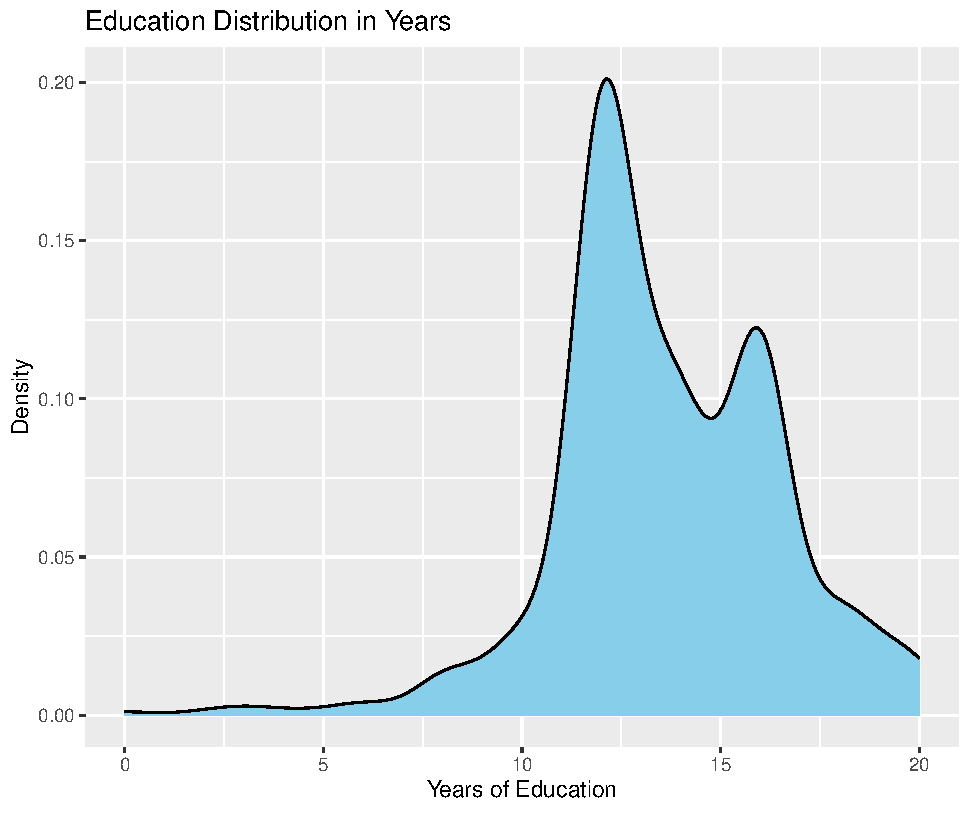
\includegraphics[width=0.4\textwidth]{2_education_distribution.pdf}

The upper two graphs depicting the distribution of recipient age and education, 
notable patterns emerge. The predominant age group among recipients falls within the range 
of 25 to 50 years. Simultaneously, a significant proportion of recipients possess either 
12 or 16 years of education, pointing towards a prevalence of high school or university graduates 
within the dataset. This observation highlights the demographic composition of the majority of recipients, 
indicating a concentration of individuals who have completed their education at either the high school or university level.
\newline

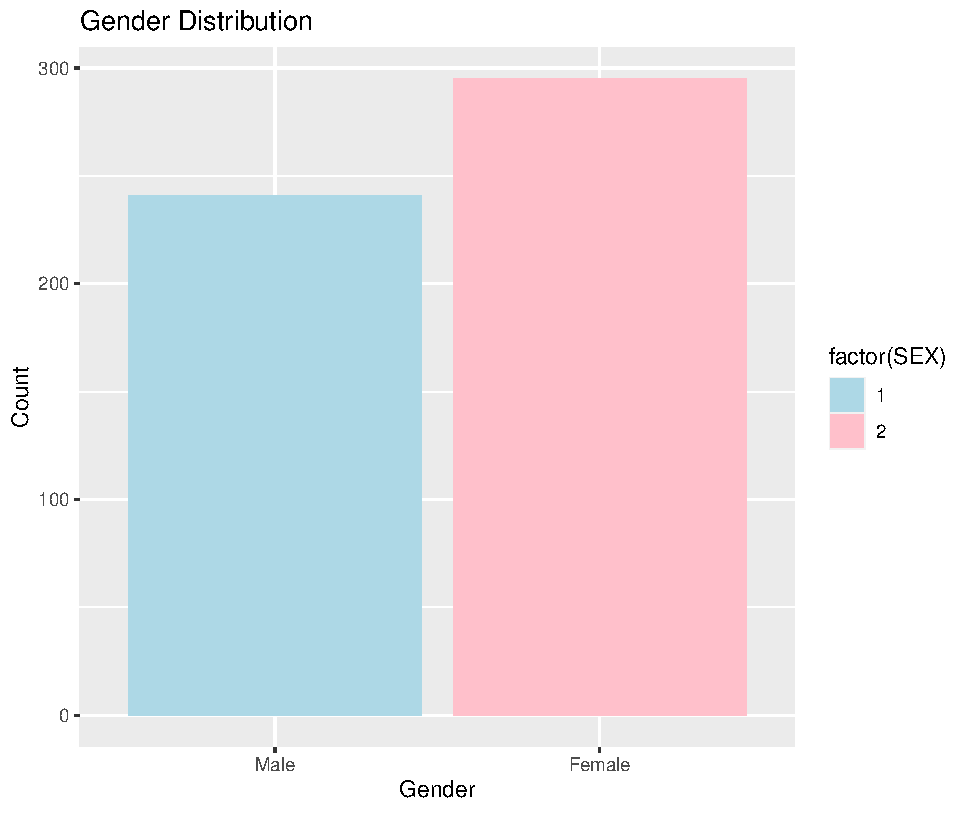
\includegraphics[width=0.4\textwidth]{3_gender_distribution.pdf}

The above graph simply showcase the distribution of gender within the dataset. Which we can 
see that the number of different is not very big, indicating a farily eqaul distribution among gender.
\newline

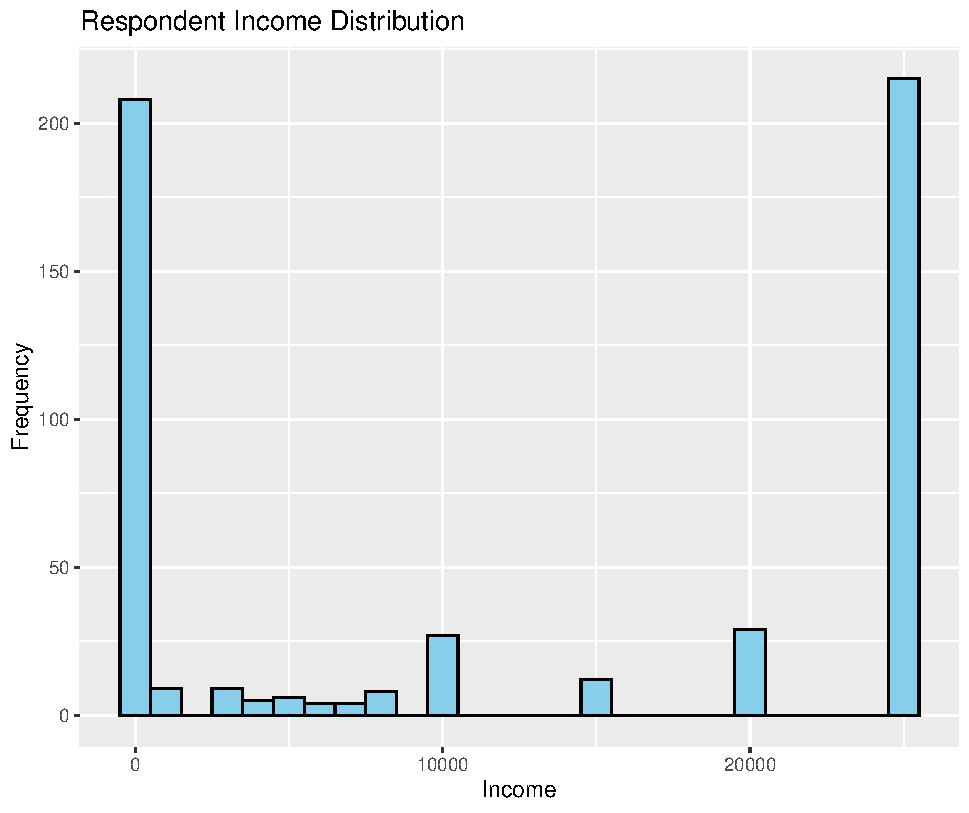
\includegraphics[width=0.4\textwidth]{5_personal_income_number.pdf}
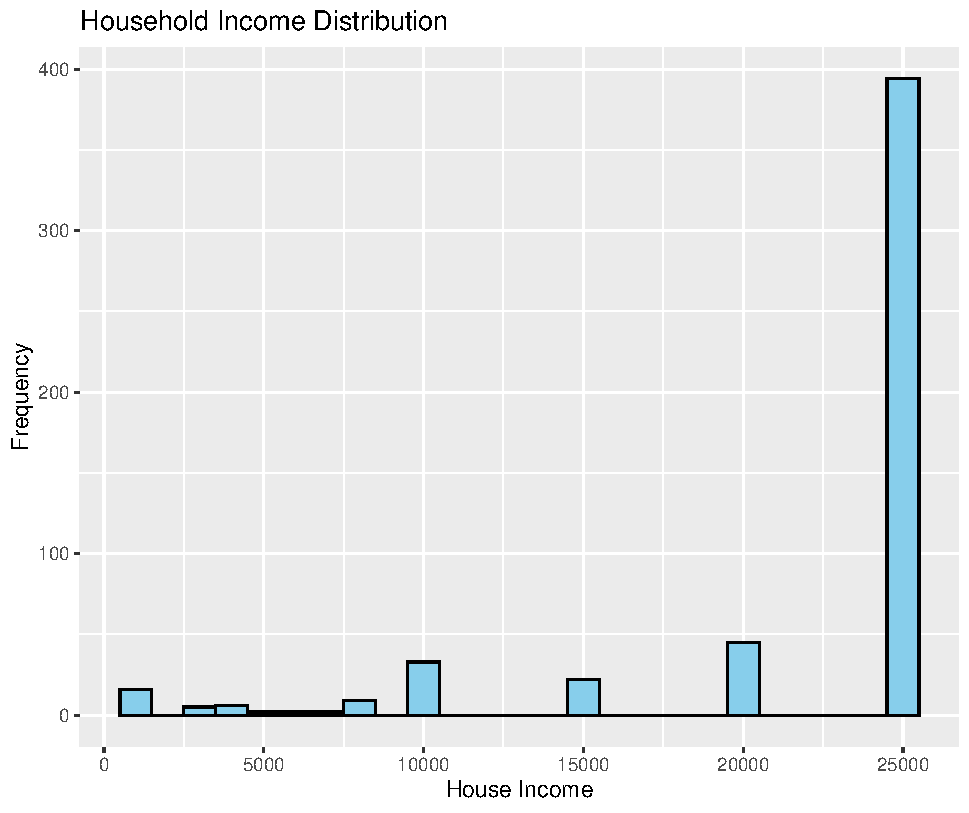
\includegraphics[width=0.4\textwidth]{7_house_income_number.pdf}

Examining the two upper graphs representing personal income and household income for each 
recipient, a noteworthy pattern emerges. It appears that the number of individuals reporting 
\$0 in income is approximately equal to those reporting incomes exceeding \$250,000. 
This observation prompts the hypothesis that individuals with high incomes may have a 
partner who stays at home and generate low or none income, although further statistical analysis is required to draw definitive conclusions.
\newline

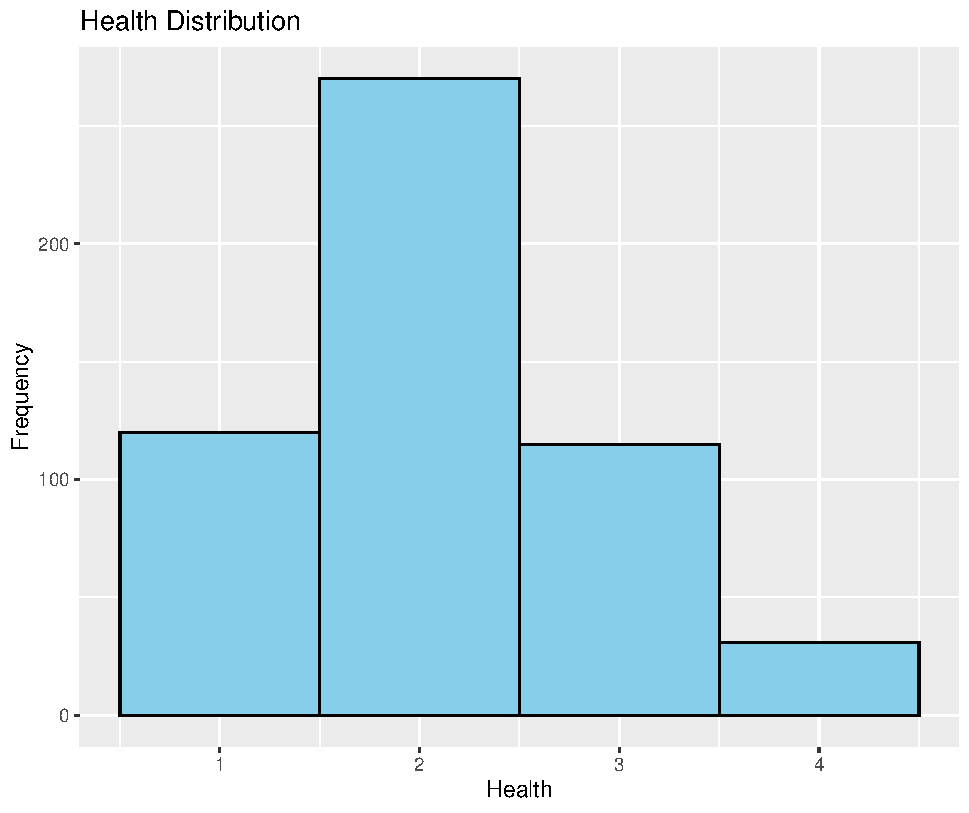
\includegraphics[width=0.4\textwidth]{8_health_distribution.pdf}
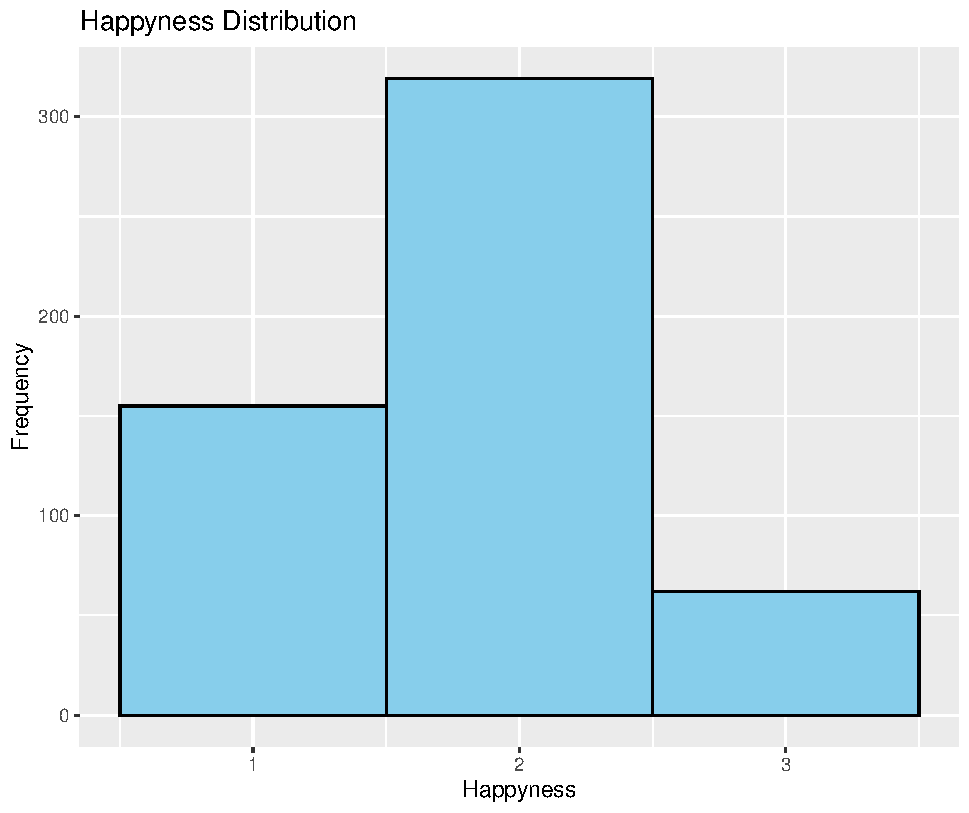
\includegraphics[width=0.4\textwidth]{9_happines_distribution.pdf}

Before making any accessment, we first have to notice that for both health and happiness, the
lower the number the better they are. So after examining the upper two graphs, it is evident that the health condition of recipients 
tends to be 2 out of 4 on the scale, which indicates a good health condition. Additionally, 
the level of happiness observed is consistently moderate, indicating a mid-level of overall well-being, 
which is pretty happy.

\section{Econometrics Models}
The econometrics that is utilized for the statistical analysis is listed below:

Model 1. $health = \beta_0 + income\beta_1 + \epsilon$

Model 2. $happy = \beta_0 + \beta_1health + \beta2income + \epsilon$

Model 3. $education = \beta_0 + \beta_1father-education + \beta_2mother-education + \beta_3spouse-education + \epsilon$

Model 4. $logincome = \beta_0 + \beta_1logspouse-income + \epsilon$

Model 5. $income = \beta_0 + \beta_1age + \beta_2education + \beta_3babies + \epsilon$

Model 6. $logincome = \beta_0 + \beta_1age + \beta_2education + \beta_3babies + \epsilon$

(The seperation of male and female dataset is utilized for Model 5 and 6.)
\newpage

\section{Estimation Results}

\begin{enumerate}
    \item[\textbf{Model 1}] $health = \beta_0 + income\beta_1 + \epsilon$

\qquad This model aim to discover the relationships between health and income. The usual assumption 
will be that for a richer person, his health condition should be better since he have access to better 
medication resources.

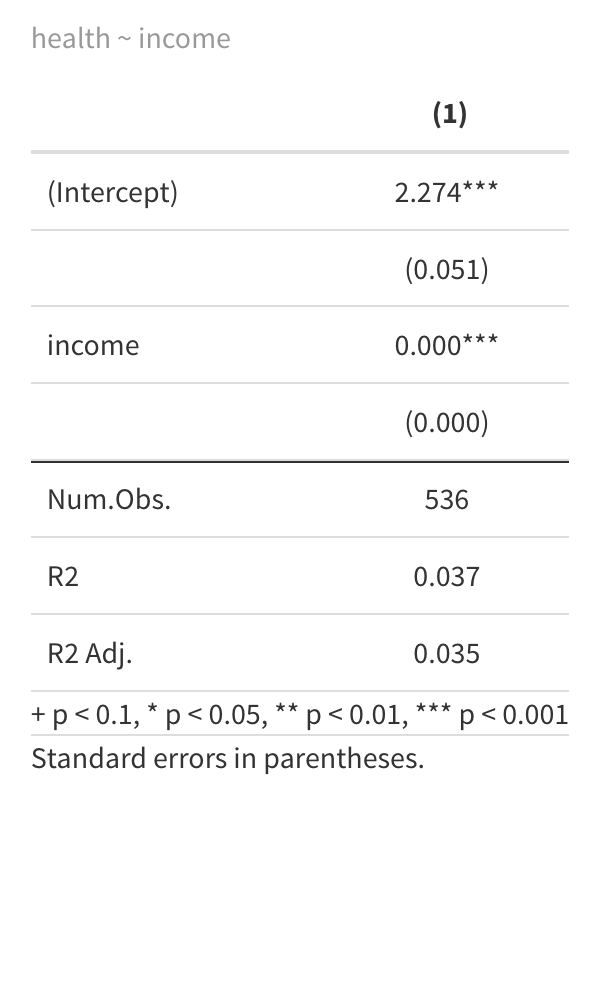
\includegraphics[width=0.3\textwidth, height=2.5in]{health~income_table.png}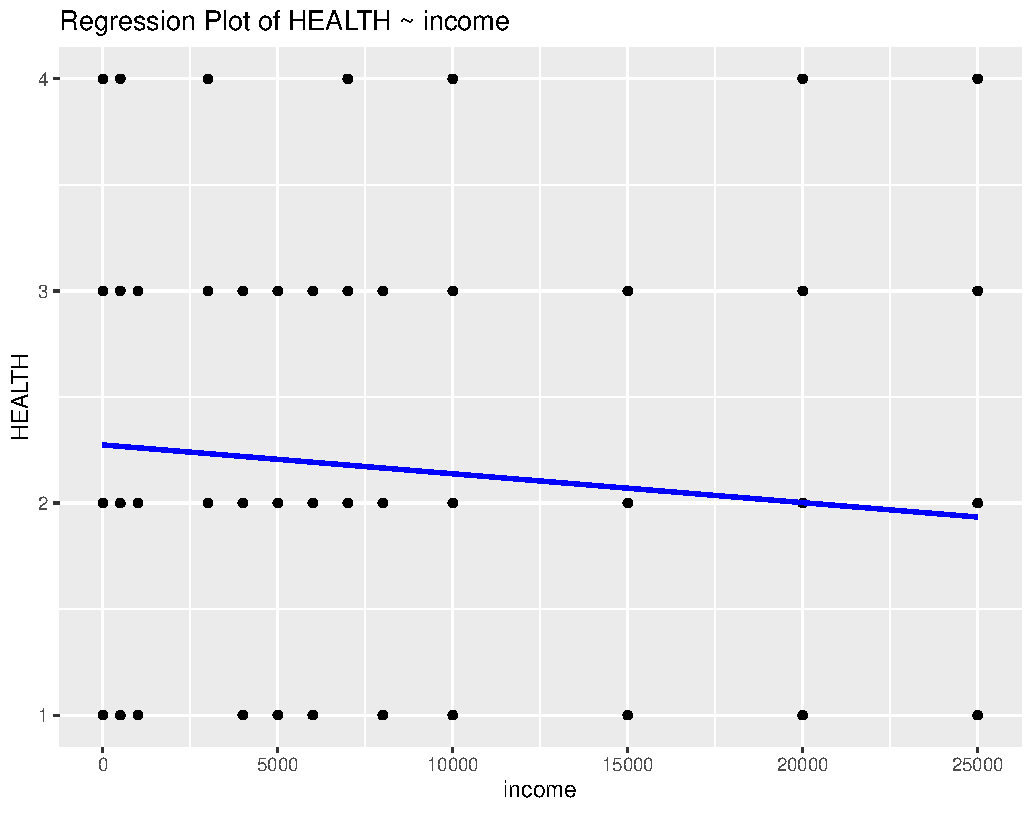
\includegraphics[width=0.5\textwidth, height=2.5in]{health~income_regression.pdf}

\qquad By inspecting the data, we can see that a person's health condition do not depend on once's income, which is different from usual assumption.

    \item[\textbf{Model 2}] $happy = \beta_0 + \beta_1health + \beta2income + \epsilon$
    
\qquad This model seeks to investigate the links between happiness, health, and income, operating on the 
assumption that individuals tend to experience greater happiness when they enjoy both financial prosperity 
and good health.

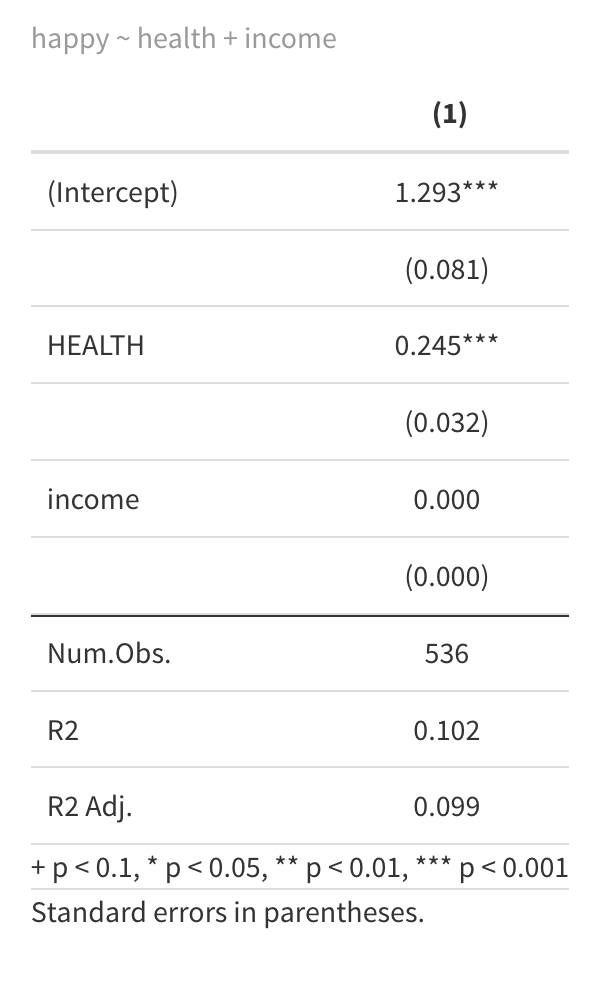
\includegraphics[width=0.3\textwidth, height=2.5in]{happy~health+income_table.png}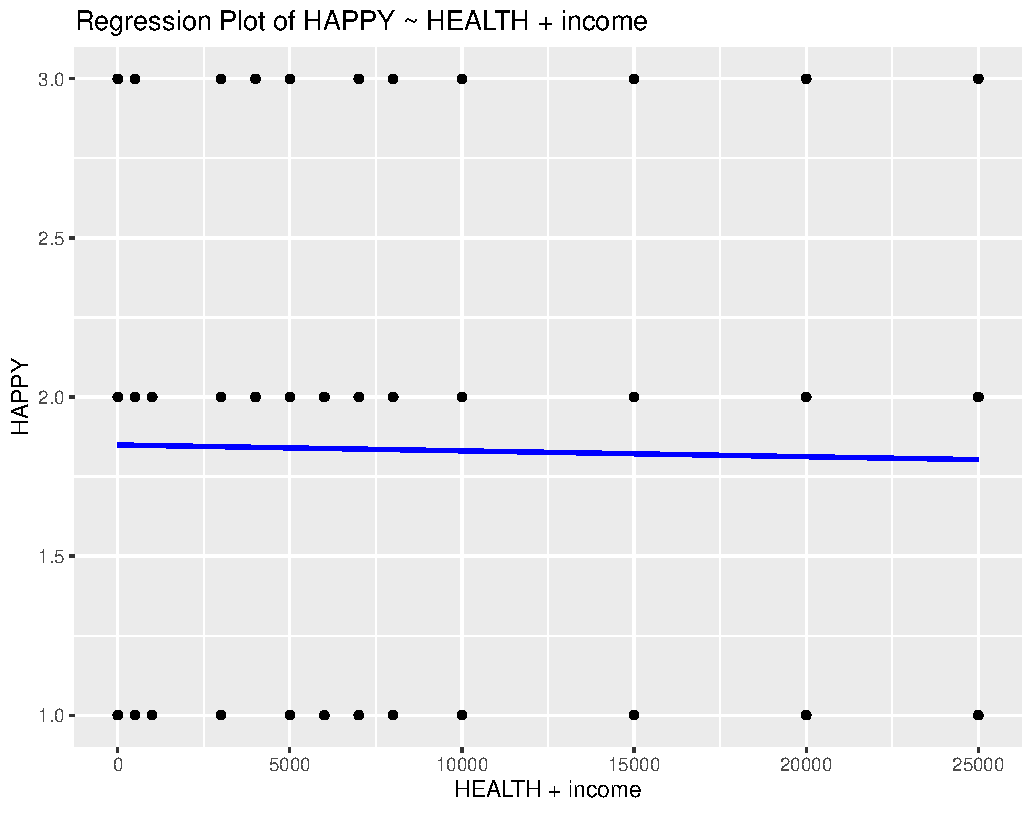
\includegraphics[width=0.5\textwidth, height=2.5in]{happy~health+income_regression.pdf}

\qquad By inspecting the table and graph, we can find out that happiness is affect by health but not income. 
More specificly, a 1 increase in scale of healthiness increase 0.245 in scale of happiness. So we can conclude that the usual assumption
is partially support by the empirical data and statistical analysis.

    \item[\textbf{Model 3}] $education = \beta_0 + \beta_1father-education + \beta_2mother-education + \beta_3spouse-education + \epsilon$
    
\qquad This model aims to explore the interconnections between an individual's educational 
attainment and the educational backgrounds of their parents and spouse. Conventionally, it's often presumed 
that there exists a strong correlation between an individual's level of education and that of their parents and spouse.

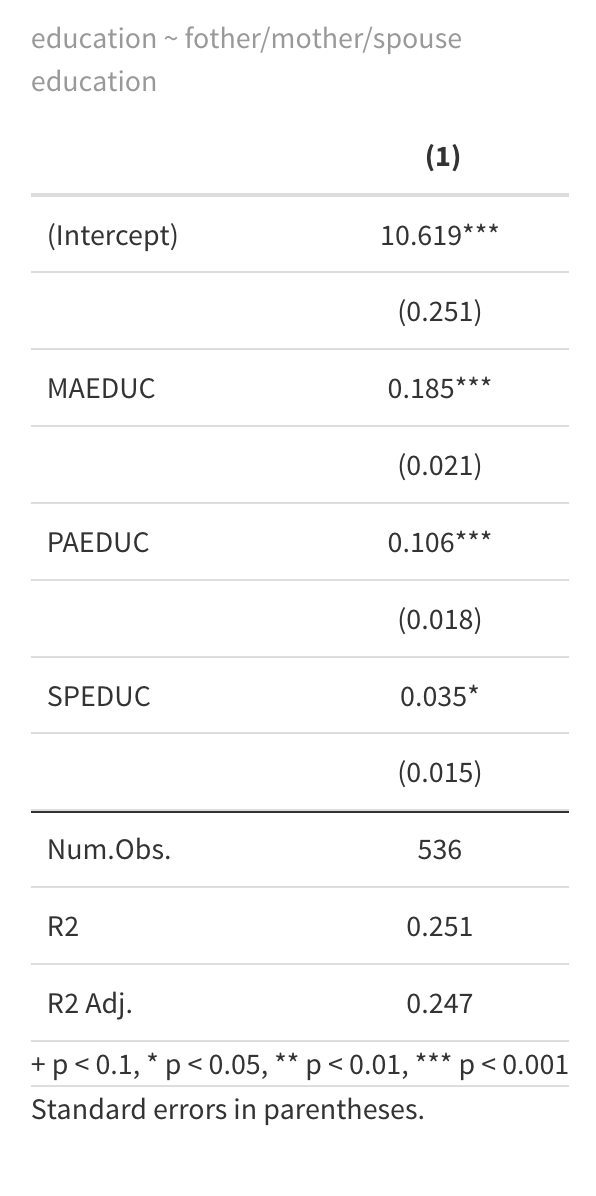
\includegraphics[width=0.3\textwidth, height=3.5in]{education_table.png}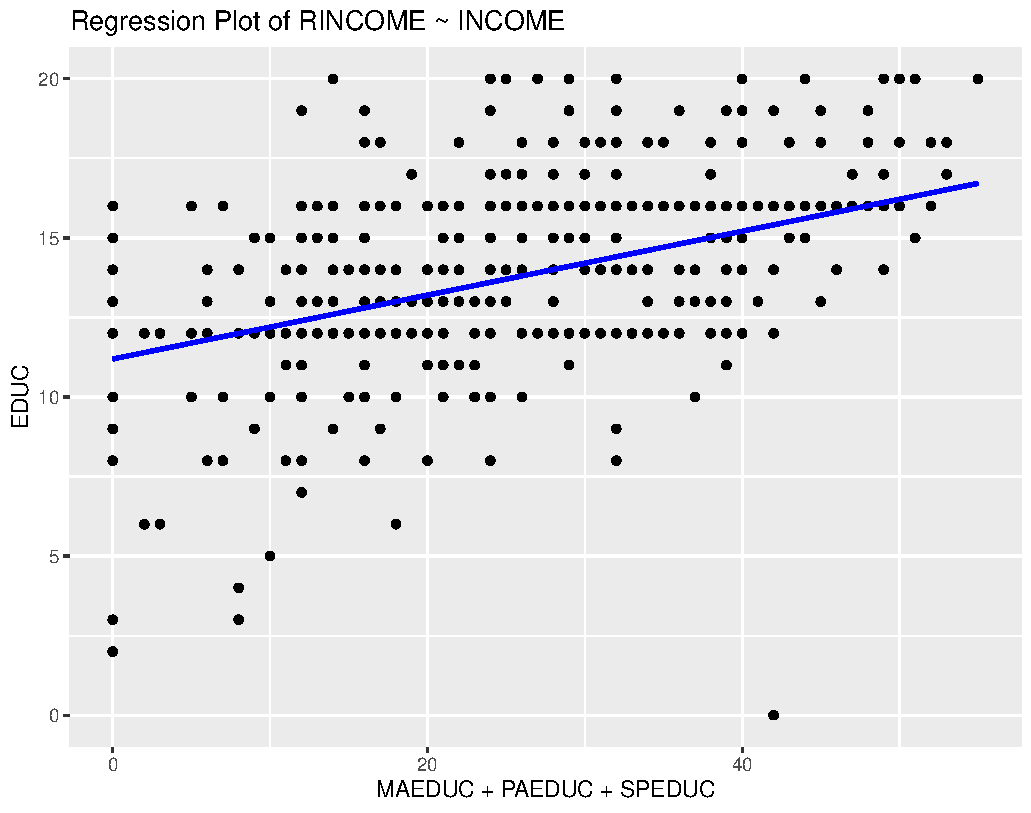
\includegraphics[width=0.5\textwidth, height=2.5in]{education_regression.pdf}

\qquad Upon examining the table, it becomes evident that there exists a strong correlation 
between an individual's level of education and that of their parents. To be precise, for each 
additional year of education attained by the mother and father, the individual's education 
increases by approximately 0.185 and 0.106 years, respectively. However, the correlation between 
an individual's education and that of their spouse appears to be relatively weak and lacks statistical significance.

    \item[\textbf{Model 4}] $logincome = \beta_0 + \beta_1logspouse-income + \epsilon$
    
\qquad This model seeks to explore the association between the logarithm of an individual's personal 
income and the logarithm of their spouse's income. Conventionally, it is assumed that higher personal 
income for one individual might correlate with their spouse having the option to be a stay-at-home parent or not work, 
thereby implying a negative correlation between the two variables.

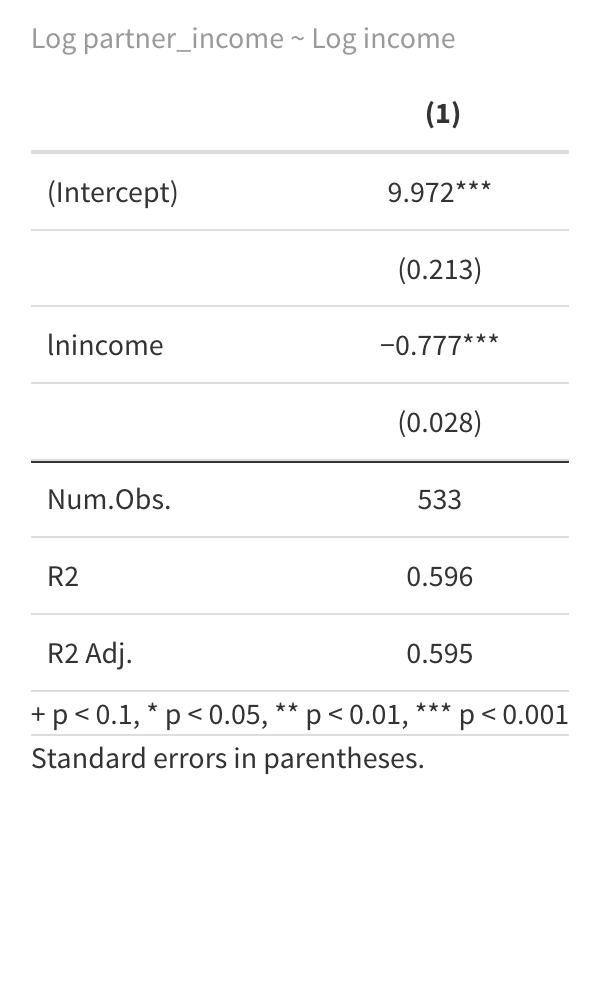
\includegraphics[width=0.3\textwidth, height=3in]{log_p_income_table.png}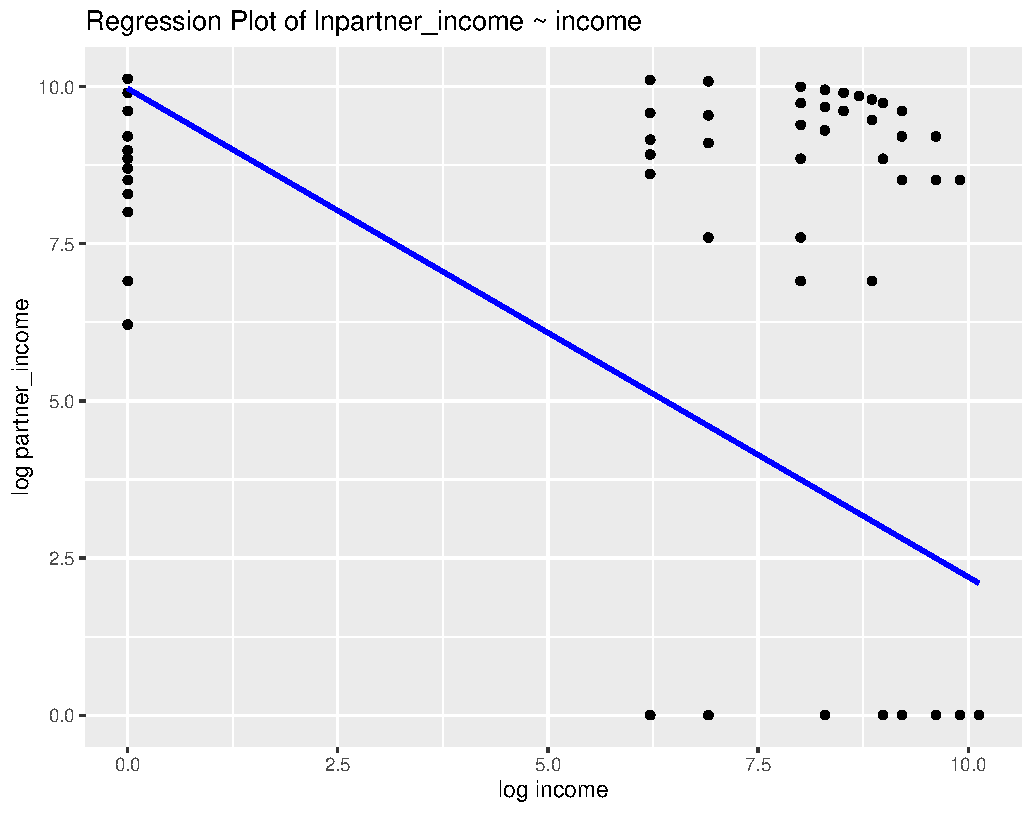
\includegraphics[width=0.5\textwidth, height=2.5in]{log_p_income_regression.pdf}

\qquad Upon inspecting the table, it becomes evident that there exists a negative correlation 
between an individual's income and that of their spouse. To be precise, for every 1\% 
increase in an individual's income, there is a corresponding decrease of 0.777\% 
in their spouse's income. This finding aligns with the conventional assumption. 
However, it is imperative to acknowledge that the dataset originates from the US government. 
Consequently, when examining countries where dual-income households constitute the predominant family structure, 
the relationship between personal income and spousal income may diverge.

    \item[\textbf{Model 5}] $income = \beta_0 + \beta_1age + \beta_2education + \beta_3babies + \epsilon$
    \item[\textbf{Model 6}] $logincome = \beta_0 + \beta_1age + \beta_2education + \beta_3babies + \epsilon$

\qquad Models 5 and 6 aim to explore the relationship between income or log-income 
and key determinants of income: age, education, and the number of dependents in the subject's 
family. According to labor economics theory, income typically exhibits a positive correlation with 
age, implying that income tends to rise as individuals age. Similarly, human capital theory suggests 
a positive relationship between income and education; individuals with higher levels of education generally 
possess greater human capital, resulting in higher earning potential. Additionally, the number of dependents 
in a family is expected to impact income, as greater financial resources are typically required to support a larger family size.
Statistical analyses using these models were conducted on three distinct datasets: male, female, and combined datasets. By examining datasets categorized by gender, we aim to uncover gender-specific insights into how various factors influence income levels.

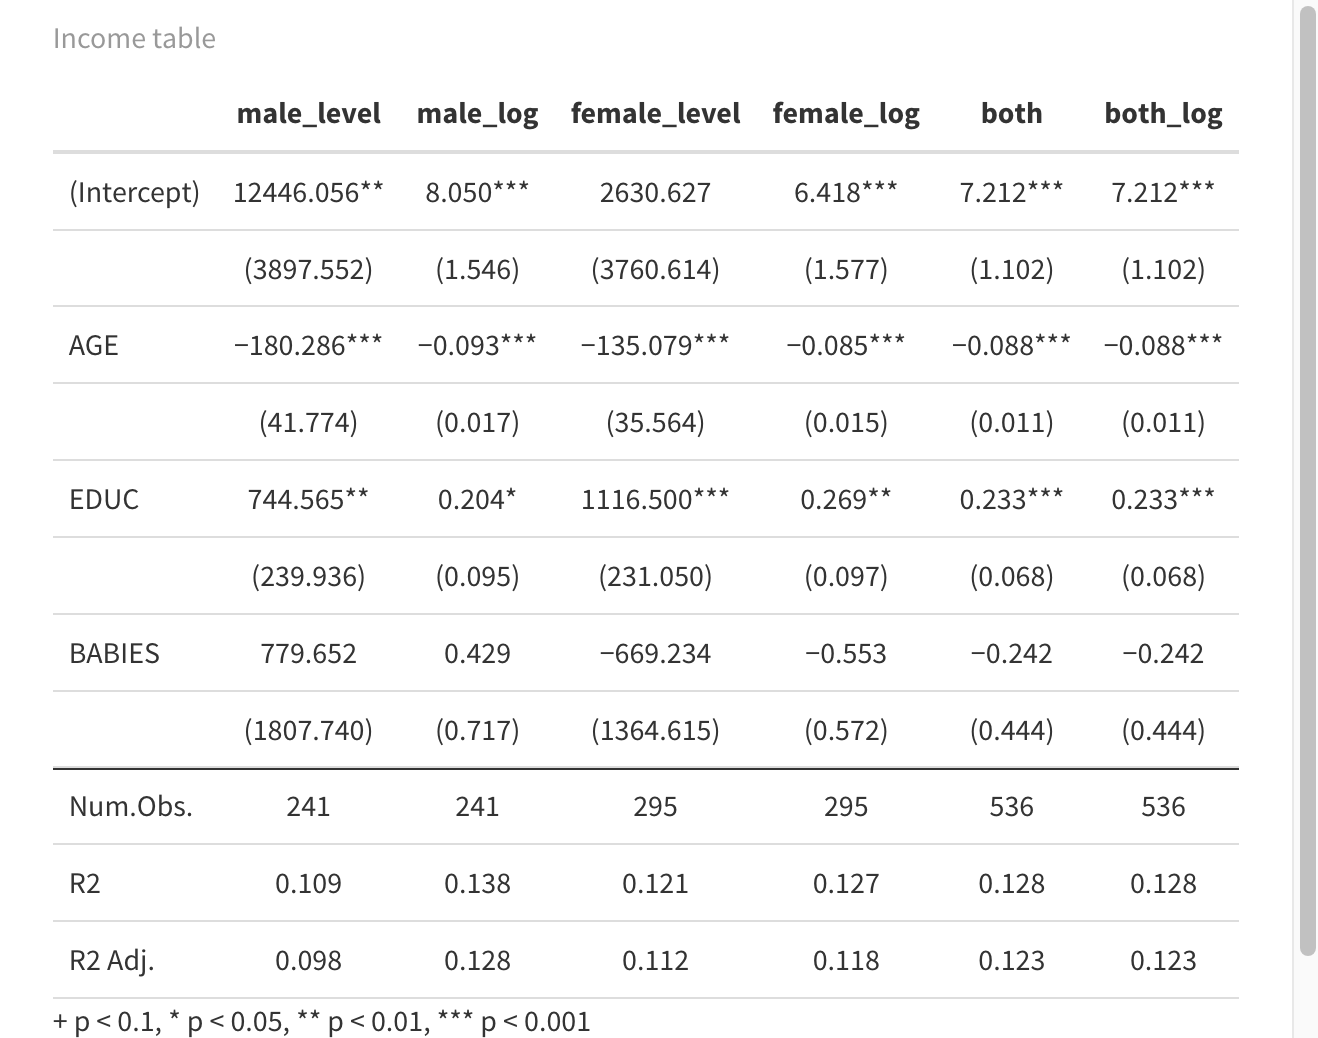
\includegraphics[width=0.95\textwidth]{income_table_big.png}
\newline

\qquad Upon inspecting the data, several conclusions become apparent. Firstly, there is a negative correlation between age and income for both males and females. Additionally, education positively correlates with income for both genders, with each additional year of education leading to substantial increases in income.
Specifically for males, a one-year increase in age corresponds to a 0.9\% decrease in income, while each additional year of education results in a significant 20.4\% increase. Furthermore, each additional baby in the family appears to positively impact male income by 42.9\%, although this effect lacks statistical significance.
In contrast, females experience similar negative correlations between age and income, albeit with more pronounced effects. A one-year increase in age corresponds to an 8.5\% reduction in income for females. Intriguingly, each additional baby in the family significantly decreases female income by 55.3\%.
Moreover, for females, each additional year of education results in a remarkable 26.9\% increase in income, surpassing the growth rate observed in males.
The disparity in the impact of children on income between genders is striking. While male income benefits from an increased number of babies, female income suffers. This observation suggests the presence of entrenched gender roles within society, influencing how family dynamics intersect with income generation.
In summary, while age and education consistently influence income levels for both genders, the divergent effects of family size underscore the complex interplay between societal norms and economic outcomes for men and women.\end{enumerate}

\section{Conclusion}

\qquad In conclusion, this paper undertook a comprehensive analysis of the `GSSdata2018' dataset, employing a 
variety of econometric models to uncover meaningful relationships among key variables. Through robust 
statistical testing, we aimed to elucidate nuanced patterns within the data, ultimately 
contributing to a deeper understanding of socio-economic dynamics in the United States. 
Our findings revealed intriguing insights into the determinants of health, happiness, educational attainment, 
and income levels.

\qquad Notably, while conventional assumptions regarding the positive relationship between income and health were 
not supported by our analysis, we discovered significant associations between education and income levels. For 
instance, each additional year of education correlated with a substantial increase in income for both males and females, 
with males experiencing a 20.4\% boost and females a remarkable 26.9\% surge. Additionally, our examination of family dynamics 
unveiled gender disparities in income outcomes, with each additional baby in the family positively impacting male income by 42.9\% 
while significantly reducing female income by 55.3\%. These findings underscore the complex interplay between individual characteristics, 
societal norms, and economic outcomes, providing valuable insights for future research and policy formulation.

\end{document}